\section{Evaluation}\label{sec:evaluation}

\subsection{Data inputs}

\textit{We discuss how an attacker can inject arbitrary bytes into receivers.  We measure the effectiveness of this approach by an overshadowing simulation.  We discuss how data can also be inserted through the mailing list}

\subsection{Security audit}
\textit{Table demonstrating which currently-active CVEs are present in the software. A discussion of legacy software and its relation to security}

\subsection{Physical-Layer Validation}

\begin{figure*}
    \centering
    \begin{subfigure}{0.49\textwidth}
        \centering
        \includegraphics[width=\textwidth]{diagrams/injection/original.jpg}
        \caption{Original image with some fires.}
        \label{fig:injection-orig}
    \end{subfigure}
    \begin{subfigure}{0.49\textwidth}
        \centering
        \includegraphics[width=\textwidth]{diagrams/injection/masked_0.jpg}
        \caption{Legitimate fires masked out.}
        \label{fig:injection-masked}
    \end{subfigure}
    \begin{subfigure}{0.49\textwidth}
        \centering
        \includegraphics[width=\textwidth]{diagrams/injection/random_combined_diagonal.jpg}
        \caption{Fires randomly injected uniformly across the map. Composite of 3 images, with intensity of the fires increasing from top to bottom.}
        \label{fig:injection-random}
    \end{subfigure}
    \begin{subfigure}{0.49\textwidth}
        \centering
        \includegraphics[width=\textwidth]{diagrams/injection/pixels_800_140.jpg}
        \caption{Fires injected at attacker-specified locations.\newline}
        \label{fig:injection-logo}
    \end{subfigure}
    \caption{An overview of the possible ways an attacker can manipulate the output of the forest fire detection algorithm by overshadowing the downlinked data. In each image, forest fires detected by the algorithm are highlighted in yellow, orange, and red in increasing order of intensity.}
    \label{fig:injection}
\end{figure*}

\begin{comment}
\begin{figure}
    \centering
    \includegraphics[width=\columnwidth]{diagrams/overshadowing_demo.pdf}
    \caption{Representation of a signal injection attack through overshadowing.}
    \label{fig:overshadowing_demo}
\end{figure}
\end{comment}

\begin{figure}
    \centering
    \includegraphics[width=\columnwidth]{diagrams/overshadowing_pipeline.pdf}
    \caption{An overview of the GNU Radio pipeline used to provide experimental validation for the overshadowing attacks. IQ samples are indicated in blue, bitstreams in magenta.}
    \label{fig:overshadowing_pipeline}
\end{figure}

In order to demonstrate the feasibility of signal injection attacks on EOS downlink systems in a real-world setting, we perform a simulated analysis of the proposed attacks.
We use ``GNU Radio'' to construct a pipeline which simulates a legitimate downlink signal broadcast from the Terra satellite and demodulated by a standard QPSK \textbf{TODO make sure explained} demodulator.
We also simulate an attacker-injected signal added to the legitimate signal and demodulated by the same process.
By varying the gain on the injected signal and measuring the Bit Error Rate (BER) of the decoded bytes, we can assess the transmission power required for the attack to succeed.
The concept of signal overshadowing is illustrated in Figure~\textbf{TODO}, and an overview of the experimental configuration is shown in Figure~\ref{fig:overshadowing_pipeline}.
The source code is also available alongside our other artifacts (\textbf{TODO}).

In order to carry out these simulations with a reasonable degree of confidence that they accurately represent the real world, we establish simulation parameters based on known characteristics of the EOS radio systems.
We use the link budget established in~\cite{quinnNew2003} to establish the Effective Isotropic Radiated Power (EIRP) and free-space path loss of the radio signals transmitted by the Aqua and Terra satellites, as well as the antenna gain for signals within the beam of the receiver, and losses within the signal processing pipeline.
We also look at the specification for a commercial EOS ground station to understand how the hardware compares to NASA's ground stations~\cite{dartcomsystemsltdXBand2021}.
On the attacker's side, we use the following standard formula for computing Free-Space Path Loss (FSPL):
\begin{align}
    \text{FSPL}_{\text{dB}} = 20\log_{10}(d) + 20\log_{10}(f) - 147.55, \label{eq:fspl}
\end{align}
where $d$ is the distance from the receiver in meters, and $f$ is the frequency in hertz.
We use the reference antenna radiation pattern given by the International Telecommunication Union in~\cite{itu2022antenna} to estimate the out-of-beam gain of the receiver to be approximately $-10.0$\,dB.
These key values are summarised in Table~\ref{tab:experimental-values}.

\begin{table}
    \resizebox{\columnwidth}{!}{%
    \begin{tabular}{lcc}
        \toprule
        & Victim & Attacker \\
        \midrule
        EIRP (dBm) & $44.4$ & $[0 \dots 100]$ \\
        Distance $d$ (km) & $\sim 713$ & $[0 \dots 10]$ \\
        Free-Space Path Loss (dB) & $179.0$ & $\text{FSPL}_{\text{dB}}(d)$ \\
        Amplitude Multiplier $\left(m = 10^{\frac{\text{EIRP}_{\text{dB}}-\text{FSPL}_{\text{dB}}}{20}}\right)$ & $1.86 \cdot 10^{-7}$ & $m$  \\
        Antenna Gain $g_A$ (dB) & $44.1$ & $-10.0$ \\
        Antenna Amplitude Multiplier $\left( m_A = 10^{\frac{g_A}{20}} \right)$ & $160$ & $0.316$ \\
        System Losses (dB) & $3.7$ & $3.7$ \\
        \bottomrule
    \end{tabular}%
    }
    \caption{Key values used in overshadowing simulations.}
    \label{tab:experimental-values}
\end{table}

We take a range of values for the signal strength at the receiver, between $-100$ and $0$\,dBm.
Received signal strength can be expressed as a function of the attacker's EIRP and distance from the receiver, enabling us to observe the bit error rate as we vary either of these parameters.
We do not accurately model system losses -- since these are consistent between the victim and attacker, we assume their effect on the outcome of the experiment is negligible.
This is verified to be the case by performing the same experiment across a range of noise values and confirming that the result changes by a negligible amount, as seen in Figure~\ref{fig:overshadowing_ber}.
For the main experiments, we set the background noise voltage to $1\,$\textmu V and the system noise to $200$\,mV, resulting in a bit error rate below the $5$\% required for the system to function.

\begin{figure}
    \centering
    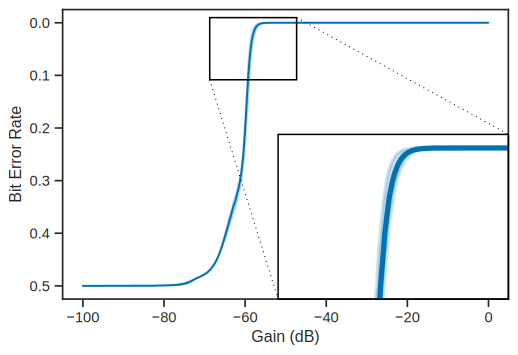
\includegraphics[width=\columnwidth]{diagrams/overshadowing_ber_2.pdf}
    \caption{Error rate of attacker-injected bits as the signal strength at the receiver increases. The small shaded region represents the range of values under different levels of background and system noise.}
    \label{fig:overshadowing_ber}
\end{figure}

The immediate results of our experiment are shown in Figure~\ref{fig:overshadowing_ber}, which compares the signal strength at the receiver to the BER of the injected signal.
In order to understand these results in a meaningful sense, we need to instead consider the factors directly controlled by the attacker: the EIRP of the transmitted signal, and the distance between the attacker and the receiver.
We take the EIRP and subtract FSPL (computed from distance using Equation~\ref{eq:fspl}) to get the received signal strength.

\begin{figure}
    \centering
    \includegraphics[width=\columnwidth]{diagrams/distance_eirp_heatmap_95.pdf}
    \caption{The bit error rate of the injected signal as the attacker varies EIRP and distance from the receiver. The values beyond which the bit error rate drops below $5$\% are indicated using a line.}
    \label{fig:distance_eirp}
\end{figure}

We see the results in Figure~\ref{fig:distance_eirp}, displaying the BER of the injected signal across a range of EIRPs and distances.
This allows us to better understand the threat model initially established in Section~\ref{sec:threat-model}.
The datasheets for the COTS radio equipment described in this section has an EIRP of up to $49$\,dBm -- we therefore know from our experimental results that an attacker with access to this equipment can carry out overshadowing attacks from a distsance of up to $0.71$\,km~\cite{endurosat:xbandtransmitter,endurosat:xbandantenna}.
With access to a more powerful amplifier, the feasible attack range can be extended significantly; an organized criminal group or nation-state level attacker could reasonably be assumed to have access to these.

We conclude from these results that there is moderate cause for concern regarding overshadowing attacks on NASA ground stations -- a motivated hobbyist with a relatively small budget can carry out attacks from a moderate distance, and attackers with greater means can do so from even further away.
Furthermore, it is difficult to prevent overshadowing attacks without some method of validating the authenticity of the received signal, and locating the attacker requires a specialized setup to triangulate the signal's origin.
This has implications beyond the attacks described in this paper, demonstrating that all downlink processing systems should be regarded as untrusted unless the data link is authenticated in some way.
